\section{Mediciones}

Se realizaron medicions en base a crear arreglos de diferentes largos, yendo de 100 en 100 elementos, donde los elementos en cada caso fueron generados por los valores pseudoaleatorios del lenguaje (el módulo \texttt{random}). 

\begin{figure}[H]
    \centering
    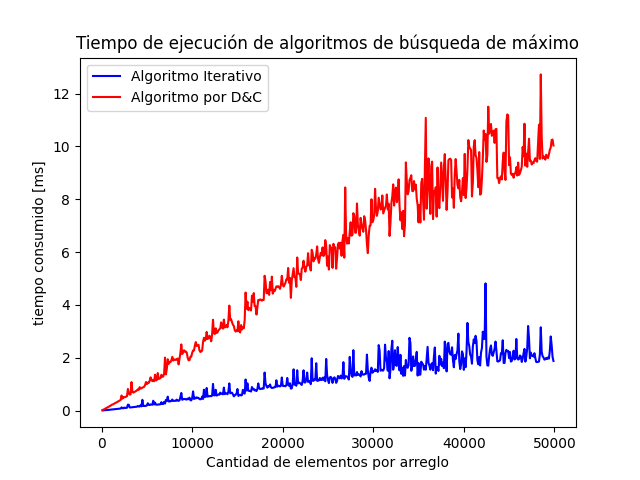
\includegraphics[width=1\textwidth]{img/tiempos.png}
\end{figure}

Como se puede apreciar, ambos algoritmos tienen una tendencia efectivamente lineal en función del tamaño de la entrada, si bien el algoritmo iterativo es más veloz en cuestión de constantes.
